% Provenance (never printed): see sources/outline_sources.md (Year 3: primordial
% nucleosynthesis and stellar burning recalled from the physics books; the s and r
% processes; supernovae and neutron-star mergers; galactic chemical evolution; from the
% solar abundances to the composition of the Earth).
% Brief: sources/book5/BRIEFS.md, ch. 30. Curves from figdata/bachelor-3/
% solar_abundances.py (Asplund, Amarsi and Grevesse 2021, Table 2), neutron_capture.py
% (their Table B.1 isotopes, KADoNiS v0.3 cross sections, IAEA Live Chart half-lives) and
% chemical_evolution.py (closed box against the Geneva-Copenhagen survey of Casagrande et
% al. 2011, and a two-phase [alpha/Fe] model). Exercise and problem values in the Book 5
% scratch calculator calc/ch30.py.
\chapter{D'où viennent les éléments}\label{ch:b3:origin-of-elements}

Le calcium d'une falaise calcaire a été produit, pour l'essentiel, dans
des étoiles massives qui ont explosé avant la naissance du Soleil. Le fer du
noyau terrestre provient surtout d'une autre sorte d'explosion, celle d'une
naine blanche. Le platine d'une bague appartient à un pic d'abondance construit
par des salves de \omterm{def:b3:origin-of-elements:s-process}{captures de neutrons} durant quelques secondes, lors de fusions de deux
étoiles à neutrons ou dans un type rare de supernova~; lequel des deux en a produit la plus grande part
reste encore débattu.
Chacun de ces événements a laissé sa marque dans la composition du Soleil,
qui est aussi, à part les quelques éléments que les planètes n'ont pas pu
retenir, la composition du Système solaire. Ce chapitre déchiffre cette
archive~: il présente les \omterm{def:b3:origin-of-elements:abundance}{abondances solaires}, rappelle comment ont été formés les éléments légers,
suit les \omterm{def:b3:origin-of-elements:s-process}{captures de neutrons} qui ont bâti les éléments lourds, repère
les sites où chaque processus opère, et modélise comment la composition d'une
galaxie évolue au fil de la vie et de la mort de ses étoiles. Il s'achève là où la géologie des
volumes précédents commence~: pourquoi la Terre, faite de la même matière que
le Soleil, est si riche en fer et si pauvre en éléments volatils.
% ledger: matteucci21:production, cowan21:rprocess, kobayashi20:origins, asplund21:fig1

\begin{recall}
La nucléosynthèse primordiale, la fusion de l'hydrogène et de l'hélium dans les étoiles,
l'énergie de liaison par nucléon et son maximum près du fer, la vallée de
stabilité, la désintégration bêta et les demi-vies, la section efficace d'une réaction,
les étoiles de la séquence principale, les géantes rouges, les naines blanches, les étoiles à neutrons et
les supernovae sont traitées dans les volumes de physique. Les classes de météorites, les chondrites
CI, la température de condensation, les éléments réfractaires et
volatils, les classes de Goldschmidt et la Terre silicatée globale sont dans le
volume de deuxième année, dans ses chapitres sur la formation des planètes et sur
les éléments dans la Terre. La structure de la Galaxie, ses disques
mince et épais, son halo et ses \omterm{def:b3:milky-way-galaxies:populations}{populations stellaires} sont dans le
chapitre précédent.
\end{recall}

\section{Les abondances solaires}\label{sec:b3:origin-of-elements:solar}

Le Soleil concentre plus de \qty{99.85}{\percent} de la masse du Système
solaire, et ses couches externes ont conservé, à part quelques éléments légers
et une lente sédimentation des éléments lourds, la composition du gaz dont
le Soleil et les planètes se sont formés. Sa composition se lit de deux manières~:
à partir des raies d'absorption de sa photosphère, et à partir des chondrites CI,
les météorites dont la composition, à l'exception des éléments les plus
volatils, est la plus proche de celle du Soleil parmi toutes les matières connues.
% ledger: asplund21:fig1, asplund21:ci

\begin{definition}[Abondance solaire~; dex]\label{def:b3:origin-of-elements:abundance}
L'\emph{abondance solaire}\index{abondance solaire} d'un élément $X$ est
le nombre de ses atomes rapporté à celui de l'hydrogène dans le Soleil,
exprimé sur une échelle logarithmique où l'hydrogène vaut $12$~:
\[
\log\varepsilon(X) = 12 + \log_{10}\frac{N_X}{N_\mathrm{H}} .
\]
Une différence d'une unité dans un tel logarithme s'appelle un
\emph{dex}\index{dex}~: deux abondances qui diffèrent de $0.3$~dex diffèrent d'un
facteur de $10^{0.3} \approx 2$. Pour une étoile, l'abondance rapportée au
Soleil s'écrit avec des crochets,
$[X/\mathrm{H}] = \log_{10}(N_X/N_\mathrm{H})_\star -
\log_{10}(N_X/N_\mathrm{H})_\odot$, et de même $[X/Y]$ pour deux
éléments quelconques.
\end{definition}

La figure ci-dessous présente les \omterm{def:b3:origin-of-elements:abundance}{abondances solaires} de la compilation récente
qui a réévalué les 83 éléments à vie longue. Le fer, à
$\log\varepsilon = 7.46$, compte un atome pour chaque \num{34700} atomes
d'hydrogène~; l'hélium en compte \num{0.0820} par atome d'hydrogène.
Plusieurs traits se détachent, et la suite du chapitre les explique.
% ledger: asplund21:abstract, asplund21:ci, data:b5-asplund21

\begin{omfigure}
\centering
\begin{tikzpicture}
\begin{axis}[width=0.95\linewidth, height=8.4cm, xmin=0, xmax=94,
  ymin=-1.8, ymax=12.8, xlabel={numéro atomique $Z$},
  ylabel={$\log\varepsilon(X)$ \;($\log\varepsilon(\mathrm{H}) = 12$)},
  tick label style={font=\scriptsize}, label style={font=\small},
  legend style={font=\scriptsize, at={(0.5,-0.17)}, anchor=north,
    legend columns=2, draw=none, cells={anchor=west},
    /tikz/every even column/.append style={column sep=1em}}]
\addplot[blue!70!black, mark=*, mark size=1.3pt, restrict x to domain=0:84]
  table[x=Z, y=logeps] {figdata/out/bachelor-3-solar_abundances-even.dat};
\addlegendentry{$Z$ pair}
\addplot[blue!70!black, mark=*, mark size=1.3pt, restrict x to domain=88:94, forget plot]
  table[x=Z, y=logeps] {figdata/out/bachelor-3-solar_abundances-even.dat};
\addplot[red!70!black, mark=o, mark size=1.4pt]
  table[x=Z, y=logeps] {figdata/out/bachelor-3-solar_abundances-odd.dat};
\addlegendentry{$Z$ impair}
\begin{scope}[font=\scriptsize]
\node[anchor=west] at (axis cs:2.2,12.2) {H};
\node[anchor=west] at (axis cs:3.0,10.9) {He};
\node[anchor=west] at (axis cs:5.6,1.0) {Li, Be, B};
\node[anchor=south] at (axis cs:8,8.95) {O};
\node[anchor=south] at (axis cs:6,8.6) {C};
\node[anchor=south, align=center] at (axis cs:26,7.75) {Fe\\[-1pt]pic};
\node[anchor=north] at (axis cs:21,2.95) {Sc};
\node[anchor=south, align=center] at (axis cs:38.5,3.05) {Sr--Zr\\[-1pt]($N = 50$)};
\node[anchor=south] at (axis cs:51.5,2.5) {Te, Xe (r)};
\node[anchor=south, align=center] at (axis cs:58.5,3.7) {Ba\\[-1pt]($N = 82$)};
\node[anchor=south] at (axis cs:76.5,1.95) {Pt (r)};
\node[anchor=south, align=center] at (axis cs:82.5,2.85) {Pb\\[-1pt]($N = 126$)};
\node[anchor=south] at (axis cs:89.6,0.15) {Th};
\node[anchor=north] at (axis cs:92,-0.7) {U};
\end{scope}
\end{axis}
\end{tikzpicture}
\par\smallskip{\small Les abondances des éléments dans le Soleil, sur une
échelle logarithmique où l'hydrogène vaut 12~: valeurs photosphériques, ou celles des
chondrites CI pour les éléments qui n'ont aucune raie photosphérique
mesurable (Asplund, Amarsi et Grevesse, 2021). Les numéros atomiques pairs et impairs
sont tracés en deux courbes. Le technétium ($Z = 43$) et le prométhium ($Z = 61$)
n'ont pas d'isotope à vie longue, pas plus que les éléments compris entre le bismuth et le
thorium.}\label{fig:b3:origin-of-elements:curve}
\end{omfigure}
% ledger: data:b5-asplund21, asplund21:fig1

\begin{enumerate}
\item L'hydrogène et l'hélium forment presque tous les atomes, mille fois
  plus que tous les autres réunis~; tous deux ont été produits lors du Big Bang, et
  une partie de l'hélium depuis lors dans les étoiles.
\item Le lithium, le béryllium et le bore, juste après l'hélium, se situent
  très loin en dessous du carbone~: le béryllium est douze millions de fois moins abondant.
\item Les abondances chutent fortement de l'oxygène vers les éléments lourds, avec
  des pics autour de l'oxygène, du fer, du baryum et du plomb, et
  de plus petits pics que la figure désigne.
\item Les éléments de numéro atomique pair sont plus abondants que leurs voisins
  impairs~: le scandium, situé entre le calcium et le titane, est environ \num{1400}
  fois plus rare que le calcium et \num{68} fois plus rare que le titane. Ceci
  est l'\emph{effet pair--impair}.
\item Au-delà du pic du fer, la courbe s'aplatit~: du fer à l'or, l'abondance
  diminue d'un facteur \num{3.5e6}, mais de l'or au plomb elle
  remonte, d'un facteur onze.
\end{enumerate}
% ledger: asplund21:fig1, data:b5-asplund21

En masse, la photosphère actuelle compte $X = 0.7438$ d'hydrogène,
$Y = 0.2423$ d'hélium et $Z = 0.0139$ pour tout le reste. Après correction
des éléments lourds qui sont descendus sous la photosphère depuis que le
Soleil s'est formé, les valeurs proto-solaires, celles du gaz dont le Soleil
est né, sont $X = 0.7121$, $Y = 0.2725$ et $Z = 0.0154$.
% ledger: asplund21:xyz

\begin{definition}[Métallicité]\label{def:b3:origin-of-elements:metallicity}
La \emph{métallicité}\index{métallicité} d'une étoile ou d'un gaz est sa
teneur en éléments plus lourds que l'hélium, appelés métaux en astronomie,
quelle que soit leur chimie~: en fraction massique $Z$, ou, comme on la
mesure le plus souvent, comme l'abondance du fer par rapport au Soleil, $[\mathrm{Fe/H}]$.
Une étoile avec $[\mathrm{Fe/H}] = -1$ possède un dixième du fer du Soleil par
atome d'hydrogène.
\end{definition}

Les deux sources des \omterm{def:b3:origin-of-elements:abundance}{abondances solaires} s'accordent remarquablement bien. La
figure ci-dessous les compare élément par élément. Pour 58 éléments, ceux
qui ne sont ni trop volatils pour les météorites ni détruits dans le Soleil,
l'écart moyen pondéré entre l'abondance photosphérique et celle des chondrites
CI est $\num[separate-uncertainty=true]{0.000 \pm 0.007}$~\omterm{def:b3:origin-of-elements:abundance}{dex}. Deux groupes
s'écartent de la droite. Les météorites contiennent bien moins d'hydrogène, d'hélium,
de carbone, d'azote, d'oxygène et de gaz nobles que le Soleil~: ces éléments
sont restés dans le gaz lorsque les solides se sont condensés. Le Soleil contient
\num{200} fois moins de lithium que les météorites~: il a détruit
\qty{99.5}{\percent} de son lithium par combustion nucléaire.
% ledger: asplund21:ci, data:b5-asplund21

\begin{omfigure}
\centering
\begin{tikzpicture}
\begin{axis}[width=0.66\linewidth, height=0.66\linewidth, xmin=-3, xmax=12.8,
  ymin=-1, ymax=12.8, xlabel={$\log\varepsilon$ dans les chondrites CI},
  ylabel={$\log\varepsilon$ dans la photosphère},
  tick label style={font=\scriptsize}, label style={font=\small},
  scatter/classes={0={mark=*, mark size=1.3pt, black!70},
    1={mark=square*, mark size=1.5pt, red!70!black},
    2={mark=triangle*, mark size=2pt, blue!70!black}}]
\addplot[black!40, dashed, domain=-1:12.8, samples=2] {x};
\addplot[scatter, only marks, scatter src=explicit symbolic]
  table[x=ci, y=phot, meta=group] {figdata/out/bachelor-3-solar_abundances-compare.dat};
\begin{scope}[font=\scriptsize, red!60!black]
\node[anchor=east] at (axis cs:8.12,12.0) {H};
\node[anchor=west] at (axis cs:1.45,10.914) {He};
\node[anchor=east] at (axis cs:7.25,8.55) {C};
\node[anchor=east] at (axis cs:6.1,7.83) {N};
\node[anchor=west] at (axis cs:8.5,8.45) {O};
\node[anchor=west] at (axis cs:-0.97,8.06) {Ne};
\node[anchor=west] at (axis cs:-0.35,6.38) {Ar};
\node[anchor=west] at (axis cs:-2.12,3.12) {Kr};
\node[anchor=west] at (axis cs:-1.8,2.22) {Xe};
\end{scope}
\node[font=\scriptsize, blue!60!black, anchor=west] at (axis cs:3.4,0.96) {Li};
\end{axis}
\end{tikzpicture}
\par\smallskip{\small Le Soleil face aux chondrites CI~: chaque point est
un élément, avec ses deux valeurs (Asplund, Amarsi et Grevesse, 2021~; l'échelle
météoritique est fixée de manière que le silicium coïncide). La droite en tirets
est l'égalité. Points noirs~: les 58 éléments qui concordent. Carrés~: l'hydrogène,
l'hélium, le carbone, l'azote, l'oxygène et les gaz nobles, que les
météorites n'ont pas conservés. Triangle~: le lithium, détruit dans le
Soleil.}\label{fig:b3:origin-of-elements:sun-ci}
\end{omfigure}
% ledger: data:b5-asplund21, asplund21:ci

L'accord est un fait d'un grand poids pour la géologie. Il signifie que les
météorites, qu'on peut analyser en laboratoire, donnent la composition du
Système solaire pour tous les éléments sauf les plus volatils~; et que le Soleil,
dont la photosphère fournit l'hydrogène, le carbone, l'azote et l'oxygène, complète
le reste. Le volume de deuxième année a bâti la composition de la Terre
globale sur ce fondement.
% ledger: asplund21:ci

\section{Les éléments légers et les étoiles}\label{sec:b3:origin-of-elements:stars}

Les volumes de physique décrivent la nucléosynthèse primordiale~: dans les trois
premières minutes, à mesure que l'Univers se refroidit, les protons et les neutrons se
combinent en deutérium, en hélium~3, en hélium~4 et en une trace de lithium~7, et rien
de plus lourd. Les abondances primordiales observées sont une fraction massique
d'hélium $Y_\mathrm{p} = \num[separate-uncertainty=true]{0.245 \pm 0.003}$, un
rapport deutérium sur hydrogène de \num{2.5e-5} et un rapport lithium sur hydrogène
de \num{1.45e-10}, ce dernier mesuré dans de vieilles étoiles pauvres en métaux du halo
galactique. Tous les autres éléments, ainsi que l'excès d'hélium du Soleil,
$0.2725 - 0.245 \approx 0.028$, ont été produits dans les étoiles.
% ledger: pdg25:bbn, asplund21:xyz

Les étoiles des volumes de physique brûlent l'hydrogène en hélium sur la
séquence principale, puis l'hélium en carbone et en oxygène en géantes rouges~; les plus
massives poursuivent, dans des coquilles autour de leur cœur, vers le néon, le magnésium,
le silicium et enfin le fer. La fusion s'arrête là, car l'énergie de liaison
par nucléon est maximale au voisinage du fer~: construire des noyaux plus lourds par
fusion absorbe de l'énergie au lieu d'en libérer. Au-delà du pic du fer, les
éléments se forment par une autre voie, la \omterm{def:b3:origin-of-elements:s-process}{capture de neutrons}, objet de la
section suivante. Le lithium, le béryllium et le bore sont fragiles~:
ils sont détruits aux températures des intérieurs stellaires, ce qui
explique que le Soleil ait brûlé presque tout son lithium, et que ces trois éléments
forment un creux dans la courbe des abondances.

\begin{definition}[Élément alpha]\label{def:b3:origin-of-elements:alpha}
Un \emph{élément alpha}\index{element alpha@élément alpha} est l'un des éléments de numéro atomique $Z$ pair
oxygène, néon, magnésium, silicium, soufre et calcium, dont les
isotopes les plus abondants ($^{16}\mathrm{O}$, $^{20}\mathrm{Ne}$,
$^{24}\mathrm{Mg}$, $^{28}\mathrm{Si}$, $^{32}\mathrm{S}$,
$^{40}\mathrm{Ca}$) ont des nombres de masse multiples de quatre, et
qui sont produits surtout dans les étoiles massives et rendus au gaz par leur
explosion en supernovae à effondrement de cœur.
\end{definition}
% ledger: matteucci21:production, data:b5-asplund21

Les pics de l'oxygène et des \omterm{def:b3:origin-of-elements:alpha}{éléments alpha}, ainsi que l'effet pair-impair,
sont les marques de ces stades de combustion~: les noyaux d'hélium s'incorporent
plus facilement aux noyaux pairs qu'aux impairs, et les noyaux
à nombre pair de protons sont plus fortement liés. Ce qu'une étoile rend
au gaz dépend de sa masse.

\begin{definition}[Rendement stellaire]\label{def:b3:origin-of-elements:yield}
Le \emph{rendement stellaire}\index{rendement stellaire} d'un élément issu d'une étoile
de masse initiale donnée est la masse de cet élément que l'étoile a
nouvellement produit et restitue au milieu interstellaire, dans ses vents et dans son
explosion finale, rapportée à la masse de l'étoile.
\end{definition}
% ledger: matteucci21:yield

Les étoiles de moins de \qty{0.8}{M_\odot} vivent plus longtemps que l'âge de
l'Univers et ne restituent rien. Les étoiles de \num{0.8} à \qty{8}{M_\odot}
restituent de l'hélium, de l'azote, du carbone et les éléments lourds du \omterm{def:b3:origin-of-elements:s-process}{processus s}
(baryum, yttrium, strontium) dans leurs vents, et finissent en naines blanches
carbone--oxygène. Les étoiles de plus de \num{8} à \qty{10}{M_\odot} produisent
surtout des \omterm{def:b3:origin-of-elements:alpha}{éléments alpha} et un peu de fer, et explosent en supernovae à effondrement de cœur.
Une naine blanche dans un système binaire serré peut exploser en supernova de type~Ia,
et de telles explosions fournissent l'essentiel du fer.
% ledger: matteucci21:production

\begin{omfigure}
\centering
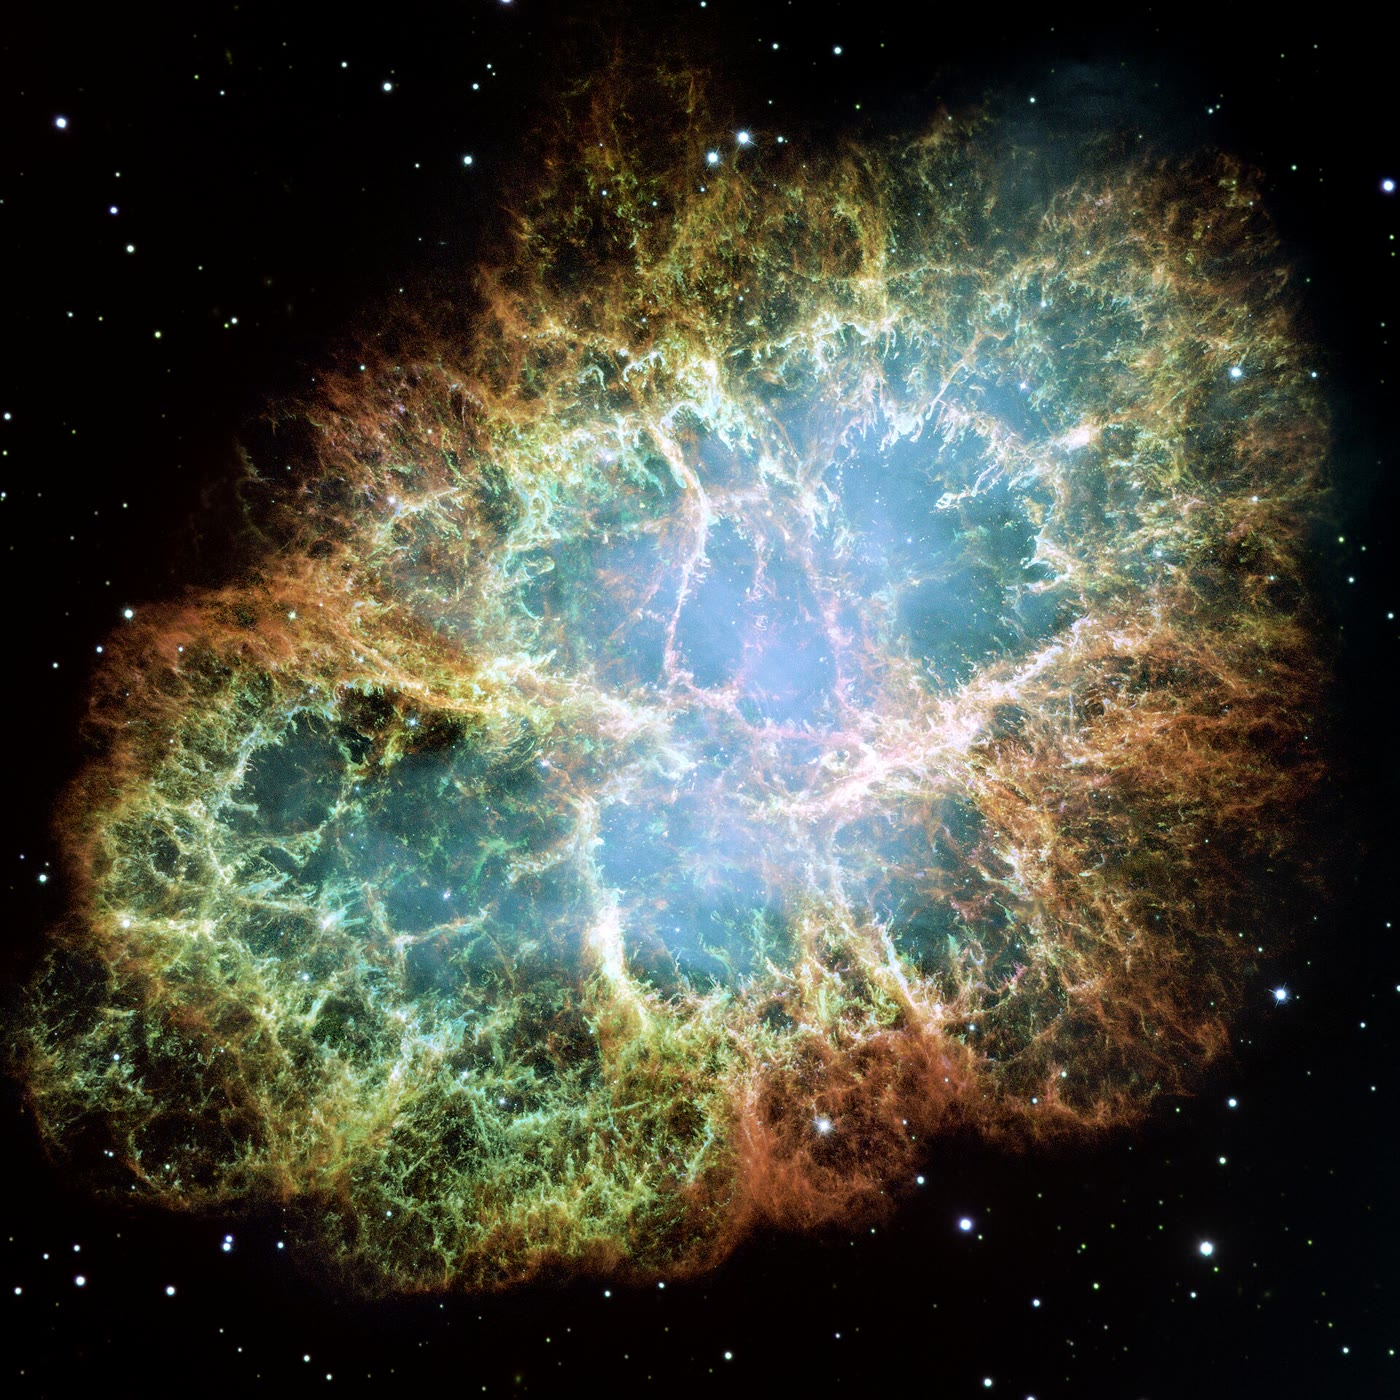
\includegraphics[width=0.5\linewidth]{images/book5/b3-crab-nebula.jpg}
\par\smallskip{\small La nébuleuse du Crabe, une mosaïque de 24 expositions du télescope
spatial Hubble~: les restes en expansion d'une étoile dont l'explosion
fut consignée par les astronomes japonais et chinois en 1054. Les filaments orangés sont les couches
externes déchiquetées de l'étoile, principalement de l'hydrogène~; la lueur bleutée à
l'intérieur provient d'électrons qui tournent en spirale autour des lignes du champ
magnétique de l'étoile à neutrons au centre, qui tourne trente fois par
seconde. Le gaz des filaments, qui porte ce que l'étoile a produit, se mélange
au milieu interstellaire. NASA, ESA, J.~Hester et A.~Loll, domaine
public.}\label{fig:b3:origin-of-elements:crab}
\end{omfigure}
% ledger: photo:b3-crab-nebula

\section{Captures de neutrons}\label{sec:b3:origin-of-elements:neutrons}

Un neutron n'a pas de charge électrique et n'est pas repoussé par un noyau~: même
un neutron lent y pénètre, et le noyau, plus lourd d'une unité de masse, évacue
l'énergie de liaison sous forme de rayon gamma. Des captures répétées produisent des
isotopes plus lourds du même élément jusqu'à ce que l'un d'eux soit instable~; il se
désintègre alors, le plus souvent par décroissance bêta-moins, en l'élément suivant, qui capture à
son tour. Les noyaux produits dépendent d'une comparaison~: le temps entre
deux captures face à la demi-vie des noyaux instables rencontrés en
chemin.

\begin{definition}[Capture de neutrons~; processus s~; processus r]\label{def:b3:origin-of-elements:s-process}
La \emph{capture de neutrons}\index{capture de neutrons} est l'absorption d'un
neutron libre par un noyau, $(Z, A) + \mathrm{n} \to (Z, A+1) + \gamma$.
Dans le \emph{processus s}\index{processus s} (lent), les captures
sont plus lentes que la plupart des décroissances bêta~: le temps entre deux captures sur un même
noyau se compte en centaines à milliers d'années, de sorte qu'un noyau instable
se désintègre presque toujours avant de pouvoir capturer, et la chaîne de captures
et de décroissances suit la vallée de stabilité. Dans le
\emph{processus r}\index{processus r} (rapide), la densité de neutrons est
si élevée que les captures sont bien plus rapides que les décroissances~: les noyaux sont
poussés vers des isotopes très riches en neutrons, loin de la stabilité, en quelques
secondes, puis se désintègrent pour revenir à la stabilité une fois les neutrons épuisés.
\end{definition}
% ledger: cowan21:timescales, cowan21:rprocess, kaeppeler11:overview

Les deux processus n'atteignent pas les mêmes noyaux, et la carte des nucléides
le montre. La figure ci-dessous en dessine une bande, du cadmium au
baryum. Le \omterm{def:b3:origin-of-elements:s-process}{processus s} la gravit le long de la vallée de stabilité~: il avance le long d'une
ligne d'un élément tant que les isotopes sont stables, puis d'un cran vers le haut par une
décroissance bêta. Le \omterm{def:b3:origin-of-elements:s-process}{processus r} vient du côté riche en neutrons, en bas
à droite~: chaque noyau très riche en neutrons se désintègre par décroissances bêta-moins successives
le long de son isobare, en conservant son nombre de masse, et s'arrête au premier
noyau stable rencontré. Un noyau stable qui possède un isobare stable de
$Z$ inférieur est \emph{protégé} du \omterm{def:b3:origin-of-elements:s-process}{processus r}~: $^{122}\mathrm{Te}$
se trouve derrière $^{122}\mathrm{Sn}$, $^{123}\mathrm{Te}$ derrière
$^{123}\mathrm{Sb}$, $^{124}\mathrm{Te}$ derrière $^{124}\mathrm{Sn}$.
Ces trois-là ne peuvent être produits que par le \omterm{def:b3:origin-of-elements:s-process}{processus s}~: ce sont des
noyaux \emph{s-seuls}. Inversement, $^{128}\mathrm{Te}$ et $^{130}\mathrm{Te}$
se trouvent au-delà du chemin s, ce qui laisse le tellure en $^{127}\mathrm{Te}$,
dont la demi-vie est de \qty{9.35}{h}~: ce sont des noyaux r-seuls.
% ledger: kaeppeler11:overview, data:b5-iaea-gs, data:b5-sigman

\begin{omfigure}
\centering
\begin{tikzpicture}
\begin{axis}[x=0.62cm, y=0.7cm, xmin=61.4, xmax=84.6, ymin=47.4, ymax=56.6,
  xlabel={nombre de neutrons $N$}, ylabel={},
  xtick={62,64,...,84}, ytick={48,...,56},
  yticklabels={Cd 48, In 49, Sn 50, Sb 51, Te 52, I 53, Xe 54, Cs 55, Ba 56},
  tick label style={font=\scriptsize}, label style={font=\small},
  axis line style={black!40}, clip=false,
  scatter/classes={0={mark=square*, mark size=6.5pt, blue!45},
    1={mark=square*, mark size=6.5pt, black!18},
    2={mark=square*, mark size=6.5pt, red!40},
    3={mark=square*, mark size=6.5pt, orange!45}}]
\addplot[only marks, mark=square, mark size=6.5pt, black!45, thin,
  restrict x to domain=61:85]
  table[x=N, y=Z] {figdata/out/bachelor-3-neutron_capture-unstable.dat};
\addplot[scatter, only marks, scatter src=explicit symbolic,
  restrict x to domain=61:85]
  table[x=N, y=Z, meta=cls] {figdata/out/bachelor-3-neutron_capture-chart.dat};
\addplot[only marks, mark=none, nodes near coords={\massnum},
  restrict x to domain=61:85,
  visualization depends on={value \thisrow{A} \as \massnum},
  nodes near coords align={center}, every node near coord/.append style={font=\tiny}]
  table[x=N, y=Z] {figdata/out/bachelor-3-neutron_capture-chart.dat};
\addplot[only marks, mark=none, nodes near coords={\massnum}, restrict x to domain=61:85,
  visualization depends on={value \thisrow{A} \as \massnum},
  nodes near coords align={center}, every node near coord/.append style={font=\tiny, black!55}]
  table[x=N, y=Z] {figdata/out/bachelor-3-neutron_capture-unstable.dat};
\addplot[quiver={u=0.48*\thisrow{dN}, v=0.48*\thisrow{dZ}}, -{Stealth[length=3pt]},
  blue!60!black, semithick, restrict x to domain=61:85]
  table[x expr=\thisrow{N0}+0.26*\thisrow{dN}, y expr=\thisrow{Z0}+0.26*\thisrow{dZ}]
  {figdata/out/bachelor-3-neutron_capture-path.dat};
\begin{scope}[red!70!black, dashed, -{Stealth[length=4pt]}, thick]
\draw (axis cs:79.1,48.9) -- (axis cs:76.4,51.6);
\draw (axis cs:81.1,48.9) -- (axis cs:78.4,51.6);
\draw (axis cs:83.1,50.9) -- (axis cs:80.4,53.6);
\end{scope}
\node[font=\scriptsize, red!70!black, anchor=south east, align=right] at (axis cs:84.5,47.5)
  {désintégrations r\\[-1pt]le long des isobares};
\end{axis}
\end{tikzpicture}
\par\smallskip{\small Une bande de la carte des nucléides, du cadmium
au baryum, nombres de neutrons 62 à 84. Les carrés colorés sont les noyaux présents dans la nature, étiquetés
par leur nombre de masse~: bleu, s-seuls~; gris, produits par les deux processus~; rouge,
r-seuls~; orange, \omterm{def:b3:origin-of-elements:p-process}{noyaux p}, atteints par aucun des deux. Les carrés ouverts sont les
noyaux instables que traverse le \omterm{def:b3:origin-of-elements:s-process}{processus s}. Flèches bleues~: le chemin s,
captures vers la droite, décroissances bêta en diagonale vers le haut et la gauche (au niveau de
$^{134}\mathrm{Cs}$ et $^{135}\mathrm{Cs}$, le chemin se divise). Flèches rouges
en pointillés~: trois des chaînes de désintégration du \omterm{def:b3:origin-of-elements:s-process}{processus r}, aboutissant à
$^{128}\mathrm{Te}$, $^{130}\mathrm{Te}$ et $^{134}\mathrm{Xe}$. Les
classes sont calculées à partir des isotopes trouvés dans la nature (Asplund,
Amarsi et Grevesse, 2021) et des demi-vies et modes de désintégration de la
carte des nucléides de l'AIEA.}\label{fig:b3:origin-of-elements:chart}
\end{omfigure}
% ledger: data:b5-sigman, data:b5-iaea-gs, data:b5-asplund21, kaeppeler11:branchings

Un troisième groupe, les carrés oranges, n'est atteint par aucun des deux processus~: les
isotopes riches en protons, comme $^{112}\mathrm{Sn}$, $^{120}\mathrm{Te}$
ou $^{124}\mathrm{Xe}$.

\begin{definition}[noyaux p]\label{def:b3:origin-of-elements:p-process}
Les \emph{noyaux p}\index{noyaux p} sont les isotopes stables du
côté riche en protons de la vallée de stabilité, au-delà du pic du fer, que
ni le \omterm{def:b3:origin-of-elements:s-process}{processus s} ni le \omterm{def:b3:origin-of-elements:s-process}{processus r} ne peuvent produire~: ils sont protégés du
\omterm{def:b3:origin-of-elements:s-process}{processus r} par un isobare stable de $Z$ plus faible et se situent hors de la voie s. Ils sont
attribués à un processus p distinct, vraisemblablement lors d'explosions de supernovae, et
à quelques exceptions près, leurs abondances sont beaucoup plus faibles que celles des
isotopes s et r voisins.
\end{definition}
% ledger: kaeppeler11:overview

La règle qui lit le tableau, appliquée aux 287 nucléides du
tableau protosolaire au-delà du zinc, trouve 30 nucléides produits uniquement par le \omterm{def:b3:origin-of-elements:s-process}{processus s}, 29 nucléides produits uniquement par le \omterm{def:b3:origin-of-elements:s-process}{processus r}
et 36 \omterm{def:b3:origin-of-elements:p-process}{noyaux p}. L'un de ces \omterm{def:b3:origin-of-elements:p-process}{noyaux p}, $^{176}\mathrm{Hf}$, est en fait
atteint par le \omterm{def:b3:origin-of-elements:s-process}{processus s} grâce à un état excité de longue durée de vie de
$^{176}\mathrm{Lu}$ que la règle simple ignore~; les 35 autres sont les \omterm{def:b3:origin-of-elements:p-process}{noyaux p}
de la littérature.
% ledger: data:b5-sigman, kaeppeler11:branchings

Le \omterm{def:b3:origin-of-elements:s-process}{processus s} peut être suivi quantitativement, car ses nucléides sont
proches de la stabilité et leurs sections efficaces de capture peuvent être mesurées. Dans un
plasma stellaire à la température $T$, les neutrons sont thermalisés, et ce qui
compte est la section efficace moyennée sur leur distribution de Maxwell--Boltzmann,
$\langle\sigma\rangle$, donnée pour une énergie thermique
$kT = \qty{30}{keV}$.
% ledger: kaeppeler11:classical

\begin{proposition}[La relation $\sigma N$]\label{prop:b3:origin-of-elements:sigma-n}
\index{relation sigma N@relation $\sigma N$}
Sur une portion de la voie s où tous les noyaux sont stables et où la
densité de neutrons $n_\mathrm{n}$ et la température sont constantes, notons $N_A$
l'abondance du noyau de nombre de masse $A$ et $\langle\sigma\rangle_A$
sa section efficace moyennée. Si le flux de neutrons a atteint un
état stationnaire, alors
\[
\langle\sigma\rangle_{A-1} N_{A-1} = \langle\sigma\rangle_A N_A ,
\]
de sorte que le produit $\sigma N$ est le même pour chaque noyau de la
portion.
\end{proposition}

\begin{proof}
Un noyau de masse $A$ \omterm{def:b3:origin-of-elements:s-process}{capture des neutrons} au taux
$\lambda_A = n_\mathrm{n}\langle\sigma\rangle_A v_T$ par noyau, où
$v_T$ est la vitesse thermique moyenne des neutrons. Il est formé par les captures sur
$A - 1$ et détruit par les captures sur lui-même, donc
$\mathrm{d}N_A/\mathrm{d}t = n_\mathrm{n} v_T\,(\langle\sigma\rangle_{A-1}
N_{A-1} - \langle\sigma\rangle_A N_A)$. En régime stationnaire, la dérivée
s'annule, ce qui donne la relation. Un noyau à grande section efficace est
vite dépassé et reste rare~; un noyau à faible section efficace
s'accumule.
\end{proof}
% ledger: kaeppeler11:classical

Les trois isotopes du tellure produits uniquement par le \omterm{def:b3:origin-of-elements:s-process}{processus s} permettent de la tester. Leurs abondances protosolaires
sont \num{0.1067}, \num{0.0373} et \num{0.1984} atomes par
million d'atomes de silicium, et leurs sections efficaces \num{295}, \num{832} et
\qty{155}{mb}~: les produits valent \num{31.5}, \num{31.0} et
\qty{30.8}{mb}, égaux à trois pour cent près, bien que les abondances
diffèrent d'un facteur cinq. Au passage d'un nombre magique de neutrons, la relation
se brise~: les noyaux à $N = 50$, $82$ ou $126$ sont si fortement liés qu'ils
capturent mal, avec $\langle\sigma\rangle = \qty{4.0}{mb}$ pour
$^{138}\mathrm{Ba}$ contre \qty{61.2}{mb} pour $^{136}\mathrm{Ba}$, et
ils jouent le rôle de goulots d'étranglement. La figure ci-dessous montre le produit pour tous les
nucléides produits uniquement par le \omterm{def:b3:origin-of-elements:s-process}{processus s}~: des paliers plats séparés par des marches près de
$A = 88$, $140$ et $208$.
% ledger: data:b5-sigman, data:b5-kadonis, kaeppeler11:classical

\begin{omfigure}
\centering
\begin{tikzpicture}
\begin{axis}[width=0.95\linewidth, height=7.4cm, xmin=60, xmax=212,
  ymode=log, ymin=1, ymax=5000, xlabel={nombre de masse $A$},
  ylabel={$\langle\sigma\rangle N$ (mb, pour $10^6$ atomes de Si)},
  tick label style={font=\scriptsize}, label style={font=\small},
  legend style={font=\scriptsize, at={(0.5,-0.17)}, anchor=north,
    legend columns=2, draw=none, cells={anchor=west},
    /tikz/every even column/.append style={column sep=1em}}]
\draw[black!35, dotted, thick] (axis cs:88,1) -- (axis cs:88,5000);
\draw[black!35, dotted, thick] (axis cs:139,1) -- (axis cs:139,5000);
\draw[black!35, dotted, thick] (axis cs:208,1) -- (axis cs:208,5000);
\addplot[blue!70!black, thick, const plot]
  table[x=A, y=sigN_model] {figdata/out/bachelor-3-neutron_capture-fitted.dat};
\addlegendentry{modèle classique ajusté pour $A > 90$}
\addplot[only marks, mark=*, mark size=1.7pt, red!70!black]
  table[x=A, y=sigN] {figdata/out/bachelor-3-neutron_capture-sigman.dat};
\addlegendentry{nucléides produits uniquement par le processus s}
\begin{scope}[font=\scriptsize]
\node[anchor=south west] at (axis cs:88.5,1.1) {$N = 50$};
\node[anchor=south west] at (axis cs:139.5,1.1) {$N = 82$};
\node[anchor=south east] at (axis cs:207.5,1.1) {$N = 126$};
\node[anchor=south] at (axis cs:123,38) {Te};
\node[anchor=south] at (axis cs:135,33) {Ba};
\node[anchor=north] at (axis cs:149,6.6) {Sm};
\node[anchor=west] at (axis cs:177,1.79) {Lu};
\node[anchor=west] at (axis cs:71,2326) {Ge};
\node[anchor=west] at (axis cs:83,428) {Kr};
\end{scope}
\end{axis}
\end{tikzpicture}
\par\smallskip{\small Produit de la section efficace de \omterm{def:b3:origin-of-elements:s-process}{capture de neutrons}
à \qty{30}{keV} (KADoNiS) et de l'abondance protosolaire (Asplund,
Amarsi et Grevesse, 2021) pour les 30 nucléides produits uniquement par le \omterm{def:b3:origin-of-elements:s-process}{processus s}. Entre les nombres magiques
de neutrons (lignes pointillées), il est presque constant~; à chacun, le flux
est freiné et le produit chute. La courbe est le modèle classique du \omterm{def:b3:origin-of-elements:s-process}{processus s}
ajusté ici aux nucléides plus lourds que $A = 90$. Les
plus légers nécessitent une seconde composante, plus faible, produite dans les
étoiles massives.}\label{fig:b3:origin-of-elements:sigma-n}
\end{omfigure}
% ledger: data:b5-sigman, data:b5-kadonis, data:b5-asplund21, kaeppeler11:classical

La courbe de la figure est le modèle classique du \omterm{def:b3:origin-of-elements:s-process}{processus s}~: une petite
fraction $G$ du fer-56 est exposée à des neutrons, les expositions étant réparties
de façon exponentielle autour d'une moyenne $\tau_0$, et le flux est suivi noyau par
noyau avec les sections efficaces mesurées. Son ajustement à 22
nucléides produits uniquement par le \omterm{def:b3:origin-of-elements:s-process}{processus s} plus lourds que $A = 90$ (en écartant $^{176}\mathrm{Lu}$, qui
se désintègre, et $^{187}\mathrm{Os}$, alimenté par la désintégration de
$^{187}\mathrm{Re}$) donne $\tau_0 = \qty{0.31}{mb^{-1}}$ et
$G = \qty{0.054}{\percent}$ du fer-56 solaire, proche des
\qty{0.04}{\percent} des analyses détaillées, dans lesquelles chaque noyau germe
capte en moyenne une quinzaine de neutrons. Les plus légers
nucléides produits uniquement par le \omterm{def:b3:origin-of-elements:s-process}{processus s}, le germanium-70 et le sélénium-76, se situent bien au-dessus de la courbe~: ils
nécessitent une seconde composante, faible, produite dans les étoiles massives.
% ledger: data:b5-sigman, kaeppeler11:classical

Lorsqu'un noyau instable sur le chemin vit à peu près aussi longtemps que le temps
entre deux captures, le flux se scinde~: une partie se désintègre, une autre capte.
De tels \emph{embranchements} se produisent pour $^{79}\mathrm{Se}$, $^{85}\mathrm{Kr}$,
$^{134}\mathrm{Cs}$, $^{147}\mathrm{Pm}$ et $^{151}\mathrm{Sm}$, parmi
d'autres. Un embranchement permet à une partie du flux de contourner un noyau~: parmi les deux
isotopes du samarium produits uniquement par le \omterm{def:b3:origin-of-elements:s-process}{processus s}, $^{150}\mathrm{Sm}$ reçoit la totalité
du flux, et $^{148}\mathrm{Sm}$ seulement la part qui a contourné le
embranchement à la masse 147, et le rapport de leurs $\sigma N$, \num{0.87},
mesure cette part. Comme celle-ci dépend de la densité de neutrons et
de la température, les embranchements sont des thermomètres et des densimètres des
étoiles où le \omterm{def:b3:origin-of-elements:s-process}{processus s} a opéré.
% ledger: kaeppeler11:branchings, kaeppeler11:pairs, data:b5-sigman

\begin{inthelab}[Mesurer une section efficace de capture]
Pour mesurer les sections efficaces moyennes dont le \omterm{def:b3:origin-of-elements:s-process}{processus s} a besoin,
les physiciens reproduisent un spectre de neutrons stellaire auprès d'un accélérateur.
Des protons frappant une cible de lithium produisent des neutrons par la réaction
$^{7}\mathrm{Li}(\mathrm{p},\mathrm{n})^{7}\mathrm{Be}$, dont le spectre
imite un spectre thermique à $kT = \qty{25}{keV}$, proche des
\qty{23}{keV} des flashs thermiques de la couche d'hélium d'une géante rouge. L'échantillon se place
juste contre la cible, dans le flux le plus intense, et après
l'irradiation, les rayons gamma des noyaux radioactifs nouvellement produits sont
comptés~: cette méthode par activation fonctionne avec des échantillons pesant moins
d'un microgramme. Lorsque le produit est stable, les neutrons sont envoyés par impulsions
et leur temps de vol sur une trajectoire donne leur énergie~; une sphère
de cristaux de fluorure de baryum entourant l'échantillon enregistre la
cascade de rayons gamma de chaque capture.
\end{inthelab}
% ledger: kaeppeler11:lab

\begin{history}[Le technétium dans les géantes rouges]
En 1952, P.~W.~Merrill repéra les raies du technétium dans les spectres des
géantes rouges de type spectral S. Le technétium n'a pas d'isotope stable~; celui
produit par le \omterm{def:b3:origin-of-elements:s-process}{processus s}, $^{99}\mathrm{Tc}$, a une demi-vie de
\num{211000} ans, bien inférieure aux durées de vie que ces étoiles
avaient déjà vécues. Le technétium a dû se former à l'intérieur des étoiles, et
récemment. Ce fut la première preuve directe que les étoiles fabriquent des éléments. En
1957, E.~M. et G.~R.~Burbidge, W.~A.~Fowler et F.~Hoyle, et
indépendamment A.~G.~W.~Cameron, formulèrent le modèle classique du
\omterm{def:b3:origin-of-elements:s-process}{processus s}.
\end{history}
% ledger: kaeppeler11:overview, data:b5-iaea-gs

Le \omterm{def:b3:origin-of-elements:s-process}{processus r} laisse ses propres pics. Son chemin longe la limite
d'émission de neutrons, la frontière au-delà de laquelle un noyau ne peut plus retenir un neutron supplémentaire,
et le flux s'attarde sur les noyaux à couches neutroniques fermées, $N = 50$, $82$ et
$126$, jusqu'à leur désintégration bêta. Ces points d'attente accumulent de la matière~;
après les dernières désintégrations vers la stabilité, les amas se situent à des nombres de masse inférieurs de quelques
unités à ceux des pics du \omterm{def:b3:origin-of-elements:s-process}{processus s} pour ces mêmes nombres magiques, qui
sont formés de noyaux stables~: vers $A = 130$ (tellure et xénon) et
$A = 195$ (platine), contre $A = 138$ et $208$ pour les pics s
du baryum et du plomb. La courbe d'abondance montre les deux séries de pics côte
à côte. Le \omterm{def:b3:origin-of-elements:s-process}{processus r} fabrique près de la moitié des éléments lourds, le \omterm{def:b3:origin-of-elements:s-process}{processus s}
l'autre moitié.
% ledger: cowan21:rprocess, kaeppeler11:overview, kaeppeler11:classical

\section{Où se déroulent les processus}\label{sec:b3:origin-of-elements:sites}

Le \omterm{def:b3:origin-of-elements:s-process}{processus s} principal se déroule dans les géantes rouges pouvant atteindre environ trois masses solaires, vers
la fin de leur vie, en tant qu'étoiles de la branche asymptotique des géantes. Entre les flashs
de combustion de l'hélium dans une couche entourant leur cœur, une fine couche riche en
carbone-13 se forme~; vers \qty{9e7}{K}, la réaction
$^{13}\mathrm{C}(\alpha,\mathrm{n})^{16}\mathrm{O}$ libère des neutrons
pendant une dizaine de milliers d'années, à des densités de $10^6$ à
\qty{e8}{neutrons.cm^{-3}}. Lors des flashs eux-mêmes, au-dessus de
\qty{2.5e8}{K}, $^{22}\mathrm{Ne}(\alpha,\mathrm{n})^{25}\mathrm{Mg}$
donne une bouffée de quelques années à \qty{e10}{cm^{-3}}. Les produits
sont ramenés à la surface, où l'on observe le technétium, puis
soufflés par le vent de l'étoile. Le \omterm{def:b3:origin-of-elements:s-process}{processus s} faible, qui fabrique les
nucléides produits uniquement par le \omterm{def:b3:origin-of-elements:s-process}{processus s} plus légers que $A = 90$, se déroule dans les étoiles massives pendant leurs combustions de l'hélium et
du carbone.
% ledger: kaeppeler11:sources, kaeppeler11:overview

Les supernovae à effondrement de cœur, fin des étoiles de plus de huit à dix
masses solaires, restituent les \omterm{def:b3:origin-of-elements:alpha}{éléments alpha} et une partie du fer peu après la
naissance des étoiles, car les étoiles massives vivent peu de temps. Les supernovae de type~Ia,
naines blanches qui explosent dans des systèmes binaires, restituent l'essentiel du
fer, mais seulement après un délai~: la naine blanche doit d'abord se former à partir d'une
étoile de moins de huit masses solaires, puis soit accréter de la matière prélevée sur un
compagnon jusqu'à atteindre la masse de Chandrasekhar, d'environ
\qty{1.44}{M_\odot}, ou fusionner avec une seconde naine blanche. Le \omterm{def:b3:origin-of-elements:s-process}{processus r} exige un milieu bien plus
extrême.
% ledger: matteucci21:production, matteucci21:time-delay

\begin{definition}[Fusion d'étoiles à neutrons~; kilonova]\label{def:b3:origin-of-elements:kilonova}
Une \emph{fusion d'étoiles à neutrons}\index{fusion d'étoiles à neutrons} est la
coalescence de deux étoiles à neutrons dans un système binaire serré, dont l'orbite a
rétrécie sous l'effet de l'émission d'ondes gravitationnelles. Une partie de la matière riche en
neutrons est éjectée. Une \emph{kilonova}\index{kilonova} est l'éclat transitoire
de ces éjectas, chauffés par la désintégration radioactive des noyaux
fraîchement produits par le \omterm{def:b3:origin-of-elements:s-process}{processus r}, et dure quelques jours.
\end{definition}
% ledger: cowan21:kilonova, ligo17:gw170817

Le 17 août 2017, les détecteurs d'ondes gravitationnelles ont enregistré la
spirale de deux étoiles à neutrons, GW170817, à une distance d'environ
\qty{40}{Mpc}~: deux astres de \num{1.17} à \qty{1.60}{M_\odot}, soit au total
\qty{2.74}{M_\odot}. Un sursaut gamma parvient \qty{1.7}{s} après la
fusion. Moins de onze heures plus tard, des télescopes repèrent un nouveau
point lumineux dans la galaxie NGC~4993 (figure ci-dessous). Son éclat ultraviolet
s'affaiblit en deux jours, puis, sur une dizaine de jours, sa lumière vire au rouge et à l'infrarouge.
Les modèles de cette évolution nécessitent plusieurs composantes d'éjectas, la plus rouge étant riche en
lanthanides, éléments lourds du \omterm{def:b3:origin-of-elements:s-process}{processus r} dont la dense forêt de raies
rend les éjectas opaques. La masse totale éjectée est
estimée entre \num{0.03} et \qty{0.08}{M_\odot}~: la première preuve directe que les \omterm{def:b3:origin-of-elements:kilonova}{fusions
d'étoiles à neutrons} produisent des éléments du \omterm{def:b3:origin-of-elements:s-process}{processus r}.
% ledger: ligo17:gw170817, mma17:kilonova, cowan21:kilonova

\begin{omfigure}
\centering
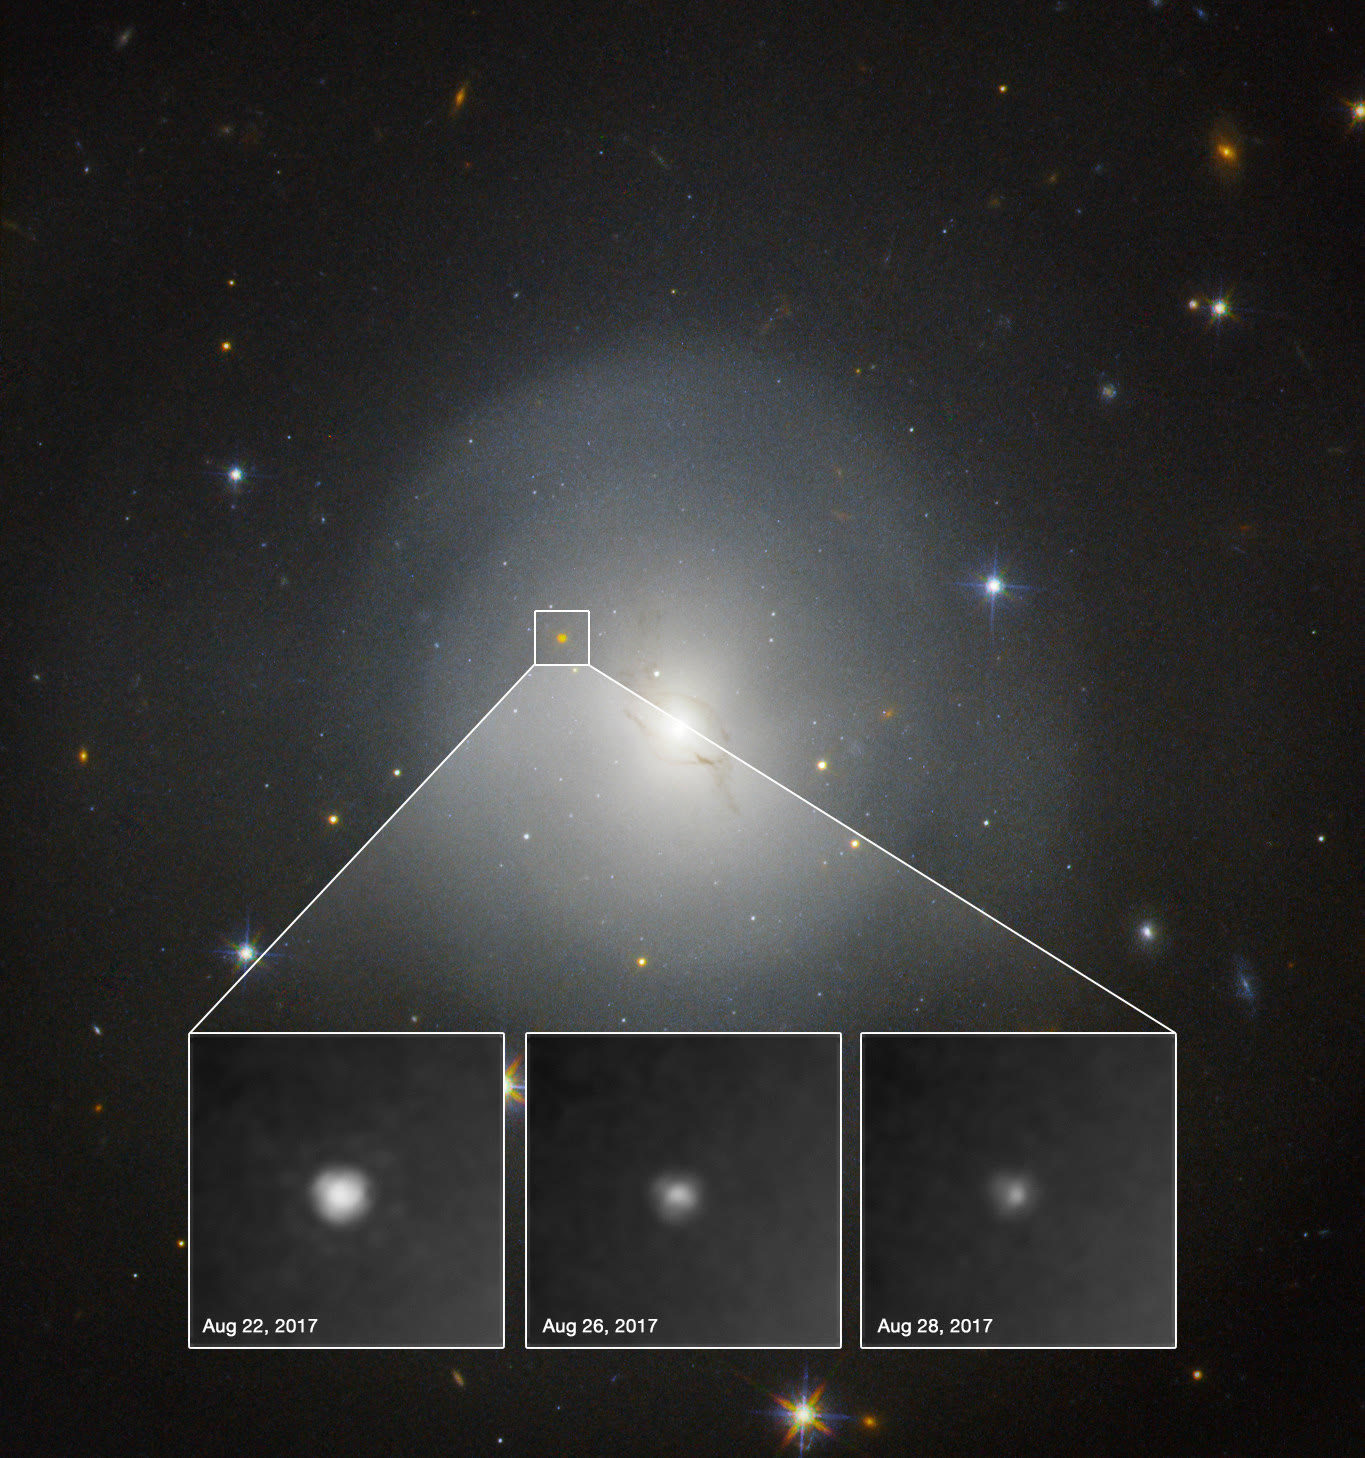
\includegraphics[width=0.55\linewidth]{images/book5/b3-kilonova.jpg}
\par\smallskip{\small La galaxie NGC~4993 photographiée par le télescope
spatial Hubble après la fusion de deux étoiles à neutrons détectée par
ses ondes gravitationnelles le 17 août 2017. Le cadre signale la \omterm{def:b3:origin-of-elements:kilonova}{kilonova}~; les
encarts, pris les 22, 26 et 28 août, la montrent s'estompant en six jours.
NASA et ESA (A.~J.~Levan, N.~R.~Tanvir, A.~Fruchter et O.~Fox), CC
BY~4.0.}\label{fig:b3:origin-of-elements:kilonova}
\end{omfigure}
% ledger: photo:b3-kilonova

\begin{dated}{2021}
Il n'est pas établi que les \omterm{def:b3:origin-of-elements:kilonova}{fusions d'étoiles à neutrons} fournissent l'essentiel
des éléments du \omterm{def:b3:origin-of-elements:s-process}{processus r} de la Galaxie. Les fusions attendent que leurs orbites
binaires se resserrent~; des modèles de l'évolution galactique où elles
sont l'unique source produisent ces éléments trop tard pour expliquer ce qu'on
observe dans les étoiles les plus anciennes et les plus pauvres en métaux. Des supernovæ rares à effondrement de cœur,
à rotation rapide et à forts champs magnétiques, ainsi que l'effondrement d'étoiles très
massives sont les autres candidats~; un modèle de la Galaxie
explique l'europium observé si environ trois pour cent des
hypernovæ de 25 à \qty{50}{M_\odot} sont du type à
entraînement magnétique.
\end{dated}
% ledger: kobayashi20:origins, cowan21:rprocess

\section{L'évolution chimique de la Galaxie}\label{sec:b3:origin-of-elements:gce}

Chaque génération d'étoiles restitue au gaz une partie de ce qu'elle a fabriqué, et
la génération suivante se forme à partir de ce gaz enrichi. La composition d'une
étoile garde donc la trace de la composition du gaz à sa naissance, et les
étoiles d'une galaxie, classées par âge, en racontent l'histoire.

\begin{definition}[Évolution chimique de la Galaxie]\label{def:b3:origin-of-elements:gce}
\emph{évolution chimique de la Galaxie}\index{evolution@évolution chimique de la Galaxie}
est la modification de la composition du gaz et des étoiles d'une
galaxie au cours du temps, sous l'action combinée de la formation stellaire, des
\omterm{def:b3:origin-of-elements:yield}{rendements stellaires}, des durées de vie des étoiles et du gaz qui entre dans
la galaxie ou en est expulsé~; et l'étude de cette modification au moyen de
modèles confrontés aux abondances d'étoiles d'âge connu.
\end{definition}
% ledger: matteucci21:simple

Le modèle le plus simple traite une région de galaxie comme une seule boîte de
gaz bien mélangée qui se transforme lentement en étoiles. Notons $s$ la masse piégée dans
les étoiles de longue durée de vie et dans les résidus stellaires, $M_\mathrm{g}$ la masse de
gaz, et $M = M_\mathrm{g} + s$ la masse totale. Le \emph{rendement par
génération stellaire} $y$ est la masse de métaux nouveaux qu'une génération d'étoiles
restitue au gaz par unité de masse qu'elle piège.
% ledger: matteucci21:yield

\begin{theorem}[Modèle de la boîte fermée]\label{thm:b3:origin-of-elements:closed-box}
\index{modèle de la boîte fermée}
Considérons une région qui n'échange aucun gaz avec son environnement, qui part
d'un gaz pur, sans métaux, qui reste bien mélangée et dans laquelle les étoiles qui
fabriquent des métaux meurent aussitôt, tandis que les autres vivent éternellement (recyclage
instantané). Alors la \omterm{def:b3:origin-of-elements:metallicity}{métallicité} du gaz vaut
\[
Z = y \ln\frac{1}{\mu}, \qquad \mu = \frac{M_\mathrm{g}}{M},
\]
où $\mu$ est la fraction de gaz, et la masse d'étoiles formées avec une
\omterm{def:b3:origin-of-elements:metallicity}{métallicité} inférieure à $Z$ vaut \mbox{$M\,(1 - \mathrm{e}^{-Z/y})$}.
\end{theorem}

\begin{proof}
Lorsqu'une masse $\mathrm{d}s$ est piégée dans des étoiles, le gaz perd
$\mathrm{d}s$, avec les métaux qu'il contient, $Z\,\mathrm{d}s$,
et gagne $y\,\mathrm{d}s$ de métaux nouveaux~:
$\mathrm{d}M_\mathrm{g} = -\mathrm{d}s$ et
$\mathrm{d}(Z M_\mathrm{g}) = (y - Z)\,\mathrm{d}s$. En développant la
seconde, $M_\mathrm{g}\,\mathrm{d}Z + Z\,\mathrm{d}M_\mathrm{g} =
y\,\mathrm{d}s - Z\,\mathrm{d}s$, et les termes en $Z$ se simplifient~:
$M_\mathrm{g}\,\mathrm{d}Z = -y\,\mathrm{d}M_\mathrm{g}$. En intégrant
depuis $M_\mathrm{g} = M$, $Z = 0$, on obtient $Z = y\ln(M/M_\mathrm{g})$. Les
étoiles formées tant que la \omterm{def:b3:origin-of-elements:metallicity}{métallicité} du gaz était inférieure à $Z$ sont celles formées
pendant que le gaz passait de $M$ à $M\mathrm{e}^{-Z/y}$, soit une masse
$M(1 - \mathrm{e}^{-Z/y})$.
\end{proof}
% ledger: matteucci21:simple

Le modèle prédit la distribution de \omterm{def:b3:origin-of-elements:metallicity}{métallicité} des étoiles de longue durée de vie.
Dans le voisinage solaire, la densité surfacique de gaz vaut
\qty{13.7}{M_\odot.pc^{-2}}, et celle des étoiles et des résidus stellaires
\qty{33.4}{M_\odot.pc^{-2}}, d'où $\mu = 13.7/47.1 = 0.29$. Si le gaz
actuel a la \omterm{def:b3:origin-of-elements:metallicity}{métallicité} proto-solaire $Z = 0.0154$, le rendement vaut
$y = 0.0154/\ln(1/0.29) = 0.0125$, et la fraction de toutes les étoiles
formées jusqu'ici dont le $Z$ est inférieur à un dixième de la valeur actuelle,
$[\mathrm{Fe/H}] < -1$ si le fer suit les métaux, est
$(1 - 0.29^{0.1})/(1 - 0.29) = 0.16$.
% ledger: mckee15:surface, asplund21:xyz, data:b5-gce

\begin{omfigure}
\centering
\begin{tikzpicture}
\begin{axis}[width=0.95\linewidth, height=7.2cm, xmin=-1.6, xmax=0.7,
  ymin=0, ymax=1500, xlabel={$[\mathrm{Fe/H}]$},
  ylabel={nombre d'étoiles par \num{0.1}~dex},
  tick label style={font=\scriptsize}, label style={font=\small},
  legend style={font=\scriptsize, at={(0.5,-0.17)}, anchor=north,
    legend columns=3, draw=none, cells={anchor=west},
    /tikz/every even column/.append style={column sep=1em}}]
\addplot[ybar, area legend, bar width=0.085, fill=black!25, draw=black!50, bar shift=0pt]
  table[x=feh, y=n_obs] {figdata/out/bachelor-3-chemical_evolution-mdf.dat};
\addlegendentry{naines F et G (6670)}
\addplot[ybar, area legend, bar width=0.085, fill=blue!55, draw=blue!70!black, bar shift=0pt]
  table[x=feh, y=n_low] {figdata/out/bachelor-3-chemical_evolution-mdf.dat};
\addlegendentry{au plus \qty{1}{M_\odot} (902)}
\addplot[red!75!black, very thick, const plot mark mid]
  table[x=feh, y=model] {figdata/out/bachelor-3-chemical_evolution-mdf.dat};
\addlegendentry{boîte fermée}
\draw[black!50, dashed] (axis cs:-1,0) -- (axis cs:-1,1500);
\node[font=\scriptsize, anchor=north west, align=left] at (axis cs:-1.57,1450)
  {boîte fermée~: \qty{16}{\percent}\\sous $-1$~;\\observé~: \qty{0.4}{\percent}};
\end{axis}
\end{tikzpicture}
\par\smallskip{\small Le \omterm{def:b3:origin-of-elements:g-dwarf}{problème des naines G}. Barres~: les \omterm{def:b3:origin-of-elements:metallicity}{métallicités} des
naines F et G du voisinage solaire (relevé de Genève--Copenhague,
échantillon à la meilleure photométrie réanalysé par Casagrande et al.,
2011), toutes les étoiles en gris, celles d'au plus une masse solaire, les étoiles de longue durée de vie
étoiles que le modèle compte, en bleu. Courbe~: la boîte fermée
avec la fraction de gaz actuelle du voisinage solaire, normalisée au
même nombre d'étoiles~; elle ne produit aucune étoile plus riche que son gaz actuel,
supposé solaire. La boîte prédit une longue queue d'étoiles pauvres en
métaux qui n'existe pas.}\label{fig:b3:origin-of-elements:g-dwarf}
\end{omfigure}
% ledger: data:b5-gcs, casagrande11:gcs, data:b5-gce, mckee15:surface

\begin{definition}[Problème des naines G]\label{def:b3:origin-of-elements:g-dwarf}
Le \emph{problème des naines G}\index{problème des naines G} désigne le manque
d'étoiles pauvres en métaux et de longue durée de vie dans le voisinage solaire
par rapport à la prédiction du \omterm{thm:b3:origin-of-elements:closed-box}{modèle de la boîte fermée}~: bien moins
de naines de type spectral G, de longue durée de vie, ont des \omterm{def:b3:origin-of-elements:metallicity}{métallicités} plus
faibles que celles qu'une boîte fermée aurait produites.
\end{definition}
% ledger: matteucci21:simple

Sur les 6670 étoiles de l'échantillon, 26 ont $[\mathrm{Fe/H}] < -1$~:
\qty{0.4}{\percent}, contre \qty{16}{\percent} pour la boîte fermée.
Même parmi les 902 étoiles d'au plus une masse solaire, la comparaison la plus
équitable~: les 26 représentent \qty{2.9}{\percent}. La sortie consiste à ouvrir la
boîte~: si le disque du voisinage solaire s'est formé par un lent apport
de gaz pauvre en métaux pendant plusieurs milliards d'années, le gaz primitif
n'a jamais constitué un grand réservoir prêt à former des étoiles pauvres en
métaux, et la queue disparaît. Les modèles du disque qui reproduisent la
distribution exigent un temps d'apport supérieur à trois à quatre milliards d'années.
% ledger: data:b5-gcs, data:b5-gce, matteucci21:simple

La seconde horloge est le rapport entre deux familles d'éléments. Les \omterm{def:b3:origin-of-elements:alpha}{éléments alpha}
proviennent des supernovae à effondrement de cœur, peu après la naissance
d'une génération stellaire~; une grande partie du fer vient des supernovae de type~Ia,
bien plus tard. Dans les vieilles étoiles du halo, avec $[\mathrm{Fe/H}] < -1$,
$[\alpha/\mathrm{Fe}]$ vaut environ $+0.4$~: ces étoiles se sont formées à partir de gaz
enrichi par les seules supernovae à effondrement de cœur. Dans les étoiles du disque, il décroît
à mesure que la \omterm{def:b3:origin-of-elements:metallicity}{métallicité} augmente, jusqu'à zéro, soit la valeur solaire, car les
supernovae de type~Ia apportent leur fer. La figure ci-dessous montre le modèle le plus simple
de ce scénario, dit du \emph{retard temporel}~: dans une boîte fermée, les deux
types de supernovae démarrent en même temps, sauf que celles de type~Ia débutent avec un retard fixe
après les premières étoiles.
% ledger: matteucci21:time-delay, matteucci21:production

\begin{omfigure}
\centering
\begin{tikzpicture}
\begin{axis}[width=0.8\linewidth, height=6.4cm, xmin=-2.4, xmax=0.25,
  ymin=-0.08, ymax=0.55, xlabel={$[\mathrm{Fe/H}]$},
  ylabel={$[\alpha/\mathrm{Fe}]$},
  tick label style={font=\scriptsize}, label style={font=\small}]
\addplot[black!40, dashed, domain=-2.4:0.25, samples=2] {0};
\addplot[blue!70!black, very thick]
  table[x=feh, y=afe] {figdata/out/bachelor-3-chemical_evolution-alpha.dat};
\addplot[only marks, mark=*, mark size=2pt, red!70!black] coordinates {(-1,0.4) (0,0)};
\node[font=\scriptsize, anchor=south, align=center] at (axis cs:-1.75,0.41)
  {supernovae à effondrement de cœur seulement};
\node[font=\scriptsize, anchor=south west, align=left] at (axis cs:-0.98,0.41)
  {Supernovae de type~Ia\\[-1pt]débutent};
\node[font=\scriptsize, anchor=south west] at (axis cs:0.01,0.01) {Soleil};
\end{axis}
\end{tikzpicture}
\par\smallskip{\small Modèle en deux phases de $[\alpha/\mathrm{Fe}]$ dans une
boîte fermée~: le plateau à $+0.4$ est le rapport produit par les supernovae à effondrement
de cœur~; les supernovae de type~Ia, qui débutent lorsque le gaz a atteint
$[\mathrm{Fe/H}] = -1$, ajoutent ensuite du fer à un rythme constant, jusqu'à ce que le rapport
soit solaire pour $[\mathrm{Fe/H}] = 0$. Le plateau et le coude sont ceux que l'on observe
dans les étoiles de la Galaxie~; la forme intermédiaire relève du modèle.
À la \omterm{def:b3:origin-of-elements:metallicity}{métallicité} solaire, \qty{60}{\percent} du fer de ce modèle
provient des supernovae de type~Ia.}\label{fig:b3:origin-of-elements:alpha}
\end{omfigure}
% ledger: data:b5-gce, matteucci21:time-delay

Les modèles détaillés de la Galaxie qui reproduisent la tendance observée
attribuent deux tiers du fer aux supernovae de type~Ia et un tiers aux supernovae
à effondrement de cœur, et trouvent que le gaz de la jeune Galaxie
a atteint $[\mathrm{Fe/H}] = -1$ en environ un à un et demi~Ga.
Le rapport sert d'horloge~: une population riche en \omterm{def:b3:origin-of-elements:alpha}{éléments alpha}
à une \omterm{def:b3:origin-of-elements:metallicity}{métallicité} donnée a formé ses étoiles vite, avant que les
supernovae de type~Ia n'ajoutent leur fer. Le \omterm{def:b3:milky-way-galaxies:structure}{disque épais} du chapitre précédent
est une telle population~: ancienne, et légèrement enrichie en \omterm{def:b3:origin-of-elements:alpha}{éléments alpha}
par rapport aux étoiles du disque mince de même \omterm{def:b3:origin-of-elements:metallicity}{métallicité}.
% ledger: matteucci21:time-delay, casagrande11:gcs

\section{Des abondances solaires à la Terre}\label{sec:b3:origin-of-elements:earth}

La Terre est faite de la même matière que le Soleil, mais non de la totalité
de celle-ci. Dans la nébuleuse en refroidissement, seuls les éléments condensés en solides
ont pu être rassemblés en planétésimaux~; le volume de deuxième année a suivi la
séquence dans laquelle ils se condensent. Le fer se condense sous forme métallique à peu près à la
même température que les silicates de magnésium, \qtyrange{1310}{1340}{K} à
\qty{e-4}{bar}, de sorte que les planètes rocheuses ont conservé leur part de fer, tandis que
l'hydrogène, l'hélium, le carbone, l'azote et les gaz nobles sont restés dans le gaz.
Dans un gaz de composition solaire, seulement environ \qty{0.5}{\percent} de la masse
se condense en roche et en métal.
% ledger: lodders:tc-table, lodders:condensates

\begin{definition}[Tendance de volatilité]\label{def:b3:origin-of-elements:volatility}
La \emph{tendance de volatilité}\index{tendance de volatilité} d'un corps planétaire
est la diminution de ses abondances, par rapport aux chondrites CI et normalisée à
un élément réfractaire, à mesure que la température de condensation diminue~: les
éléments réfractaires gardent leurs proportions chondritiques, tandis que les
éléments modérément volatils sont d'autant plus appauvris que leur température
de condensation est basse.
\end{definition}

Pour la Terre silicatée, le volume de deuxième année a tracé la tendance en fonction de la
température de condensation. Normalisé au magnésium, le zirconium
(qui se condense à \qty{1741}{K}) se situe à \num{1.11} fois sa valeur CI, le sodium
(\qty{958}{K}) à \num{0.22}, le potassium
(\qty{1006}{K}) à \num{0.19}, le rubidium (\qty{800}{K}) à \num{0.12}
et le zinc (\qty{726}{K}) à \num{0.075}. La Terre s'est formée à partir d'une matière
qui avait déjà perdu une partie de ses éléments modérément volatils avant que la
planète ne soit assemblée, ou les a perdus pendant sa croissance. Même les chondrites CI
diffèrent du Soleil d'une manière qui suit la température de condensation, quoique
faiblement~: leurs éléments modérément volatils se situent
environ \num{0.04}~\omterm{def:b3:origin-of-elements:abundance}{dex} au-dessus des valeurs photosphériques.
% ledger: lodders:tc-table, lodders:ci-table, ms95:pm-trace, asplund21:abstract

Le bilan de ce chapitre traverse donc la planète. L'oxygène,
le magnésium et le silicium du manteau sont des \omterm{def:b3:origin-of-elements:alpha}{éléments alpha} issus d'étoiles
massives~; le fer du noyau vient surtout des supernovae de type~Ia~; le thorium et l'uranium
dont la désintégration contribue à chauffer l'intérieur se situent au-delà du bismuth,
où seul le \omterm{def:b3:origin-of-elements:s-process}{processus r} parvient~; l'ensemble du mélange a été trié selon sa
volatilité avant que la Terre ne le rassemble.
% ledger: matteucci21:production, matteucci21:time-delay, kaeppeler11:overview, data:b5-sigman

\section{Exercices}

\begin{exercise}[$\star$]\label{exo:b3:origin-of-elements:1}
À partir des \omterm{def:b3:origin-of-elements:abundance}{abondances solaires} $\log\varepsilon(\mathrm{O}) = 8.69$,
$\log\varepsilon(\mathrm{Si}) = 7.51$, $\log\varepsilon(\mathrm{Fe}) =
7.46$, $\log\varepsilon(\mathrm{Au}) = 0.91$ et
$\log\varepsilon(\mathrm{Pb}) = 1.95$~: (a)~combien d'atomes de silicium et
combien d'atomes d'oxygène trouve-t-on dans le Soleil par atome de fer~? (b)~Combien d'atomes de fer
par atome d'or, et combien d'atomes de plomb par atome d'or~?
\end{exercise}

\begin{exercise}[$\star$]\label{exo:b3:origin-of-elements:2}
(a)~Combien d'atomes de fer par million d'atomes d'hydrogène le Soleil
contient-il ($\log\varepsilon(\mathrm{Fe}) = 7.46$)~? (b)~Une étoile du halo a
$[\mathrm{Fe/H}] = -2$. Combien d'atomes d'hydrogène contient-elle par atome
de fer~? (c)~Une autre étoile possède un atome de fer pour dix millions d'atomes
d'hydrogène. Quelle est sa valeur de $[\mathrm{Fe/H}]$~?
\end{exercise}

\begin{exercise}[$\star$]\label{exo:b3:origin-of-elements:3}
Les isotopes stables du xénon ont pour nombres de masse 124, 126, 128, 129, 130,
131, 132, 134 et 136. Parmi leurs isobares, le tellure ($Z = 52$) possède des
isotopes stables de nombres de masse 120, 122--126, 128 et 130~; l'iode ($Z = 53$) ne possède que le 127.
La voie s atteint le xénon en $^{128}\mathrm{Xe}$, par désintégration de
$^{128}\mathrm{I}$, et la quitte en $^{133}\mathrm{Xe}$, qui se désintègre.
Classer chaque isotope du xénon en isotope s seul, r seul, produit par les deux
processus, ou noyau p.
\end{exercise}

\begin{exercise}[$\star$]\label{exo:b3:origin-of-elements:4}
GW170817 se situe à environ \qty{40}{Mpc}, et ses rayons gamma sont arrivés
\qty{1.7}{s} après la fusion observée en ondes gravitationnelles. (a)~Depuis combien de temps
les deux signaux ont-ils voyagé~? (b)~Si le retard s'explique entièrement par
une différence entre les deux vitesses, quelle est au plus cette différence,
exprimée en fraction de la vitesse de la lumière~?
\end{exercise}

\begin{exercise}[$\star\star$]\label{exo:b3:origin-of-elements:5}
Les trois isotopes du tellure produits uniquement par le \omterm{def:b3:origin-of-elements:s-process}{processus s} ont des abondances
protosolaires de \num{0.1067}, \num{0.0373} et \num{0.1984} par $10^6$ atomes de silicium
($A = 122$, $123$, $124$) et des sections efficaces moyennes de \num{295},
\num{832} et \qty{155}{mb}. (a)~Calculer $\sigma N$ pour chacun. (b)~À partir du seul
$^{122}\mathrm{Te}$, prévoir les abondances de $^{123}\mathrm{Te}$
et de $^{124}\mathrm{Te}$, et comparer. (c)~Pourquoi la relation ne peut-elle pas
s'appliquer au $^{128}\mathrm{Te}$~?
\end{exercise}

\begin{exercise}[$\star\star$]\label{exo:b3:origin-of-elements:6}
Dans le modèle classique, chaque noyau de la voie s transmet au suivant une fraction
$f = 1/(1 + 1/(\tau_0\langle\sigma\rangle))$ du
flux, avec $\tau_0 = \qty{0.306}{mb^{-1}}$. (a)~Calculer $f$ pour
$^{124}\mathrm{Te}$ (\qty{155}{mb}) et pour le $^{138}\mathrm{Ba}$, dont le nombre de neutrons est magique
(\qty{4.0}{mb}). (b)~Les noyaux allant de
$^{137}\mathrm{Ba}$ à $^{142}\mathrm{Nd}$ sur la voie ont des sections efficaces
\num{76.3}, \num{4.0}, \num{32.4}, \num{11.0},
\num{111.4} et \qty{35.0}{mb}. De quel facteur $\sigma N$ diminue-t-il entre
$^{136}\mathrm{Ba}$ et $^{142}\mathrm{Nd}$~? (c)~Comparer avec les valeurs mesurées,
\num{27.6} et \qty{7.72}{mb}.
\end{exercise}

\begin{exercise}[$\star\star$]\label{exo:b3:origin-of-elements:7}
Un neutron d'énergie thermique $kT$ a pour vitesse
$v_T = \sqrt{2kT/m_\mathrm{n}}$, avec $m_\mathrm{n} = \qty{1.6749e-27}{kg}$.
(a)~Calculer $v_T$ pour $kT = \qty{8}{keV}$, la température de la
couche de carbone 13 d'une géante rouge. (b)~Pour $^{124}\mathrm{Te}$, avec
$\langle\sigma\rangle = \qty{155}{mb}$, calculer le temps moyen entre
deux captures, $1/(n_\mathrm{n}\langle\sigma\rangle v_T)$, pour
$n_\mathrm{n} = 10^6$, $10^8$ et \qty{e10}{cm^{-3}}. (c)~Comparer avec les
demi-vies de $^{127}\mathrm{Te}$ (\qty{9.35}{h}) et de
$^{134}\mathrm{Cs}$ (\qty{2.07}{an}). Lequel est un point de branchement~?
\end{exercise}

\begin{exercise}[$\star\star$]\label{exo:b3:origin-of-elements:8}
Dans le Soleil, $\log\varepsilon$ vaut \num{6.30} pour le calcium, \num{3.14} pour
le scandium et \num{4.97} pour le titane~; \num{1.38} pour le béryllium,
\num{2.70} pour le bore et \num{8.46} pour le carbone. (a)~Combien de fois le scandium
est-il plus rare que ses deux voisins~? (b)~Combien de fois le béryllium est-il plus rare
que le carbone~? (c)~Quel trait de la courbe d'abondance chacun illustre-t-il, et quelle
en est la cause~?
\end{exercise}

\begin{exercise}[$\star\star$]\label{exo:b3:origin-of-elements:9}
Dans le modèle à deux phases du chapitre, le palier
$[\alpha/\mathrm{Fe}] = P$ est le rapport produit par les supernovae à effondrement de cœur,
et à $[\mathrm{Fe/H}] = 0$ le rapport est solaire. (a)~Montrer que la part du fer
solaire produite par les supernovae de type~Ia vaut $1 - 10^{-P}$, et la calculer pour
$P = 0.4$. (b)~Quel palier donnerait les deux tiers des
modèles détaillés~? (c)~Une galaxie naine montre son genou à
$[\mathrm{Fe/H}] = -2$. Qu'est-ce que cela indique sur sa formation stellaire~?
\end{exercise}

\begin{exercise}[$\star\star\star$]\label{exo:b3:origin-of-elements:10}
Les chondrites CI contiennent, en parties par million en masse, \num{95870}
de magnésium, \num{3.96} de zirconium, \num{5010} de sodium, \num{530}
de potassium et \num{2.13} de rubidium~; la Terre silicatée contient
\qty{22.8}{\percent} de magnésium et \num{10.5}, \num{2670}, \num{240}
et \num{0.6} parties par million des autres. Leurs températures de
condensation à 50~\% sont \qty{1336}{K} (Mg), \qty{1741}{K} (Zr),
\qty{958}{K} (Na), \qty{1006}{K} (K) et \qty{800}{K} (Rb). (a)~Pour
chaque élément, calculer $(X/\mathrm{Mg})_\mathrm{Terre}/(X/\mathrm{Mg})_\mathrm{CI}$.
(b)~Le tracer en fonction de la température de condensation et décrire la
tendance. (c)~Pourquoi le magnésium est-il choisi comme référence~?
\end{exercise}

\begin{exercise}[$\star\star\star$]\label{exo:b3:origin-of-elements:11}
Une boîte qui fuit perd du gaz dans un vent à un taux $\lambda$ fois son taux de
formation stellaire, et n'en reçoit aucun. (a)~Montrer que sa \omterm{def:b3:origin-of-elements:metallicity}{métallicité} vaut
$Z = \frac{y}{1 + \lambda}\ln\frac{M_\mathrm{g}(0)}{M_\mathrm{g}}$.
(b)~Avec $y = 0.0125$, comparer la \omterm{def:b3:origin-of-elements:metallicity}{métallicité} atteinte lorsque le gaz n'est plus
que \qty{29}{\percent} de sa masse initiale pour $\lambda = 0$ et
$\lambda = 1$. (c)~Pourquoi les petites galaxies, à la gravité faible, tendent-elles à être
pauvres en métaux~?
\end{exercise}

\begin{exercise}[$\star\star\star$]\label{exo:b3:origin-of-elements:12}
(a)~Le Soleil a $\log\varepsilon(\mathrm{Li}) = 0.96$ dans sa photosphère
et les chondrites CI $3.25$. Calculer les deux rapports $N_\mathrm{Li}/N_\mathrm{H}$
ainsi que la fraction de son lithium que le Soleil a détruite. (b)~Les plus
anciennes étoiles pauvres en métaux présentent $N_\mathrm{Li}/N_\mathrm{H} = \num{1.45e-10}$,
tandis que la nucléosynthèse primordiale prédit \num{4.72e-10}. De quel facteur
le lithium du Système solaire dépasse-t-il chacune de ces valeurs~? (c)~Que
impliquent les deux comparaisons~?
\end{exercise}

\section{Problème~: une galaxie en boîte fermée}

\begin{problem}[{Problème du week-end --- du mélange solaire aux
métallicités des étoiles à longue durée de vie}]
\label{pb:b3:origin-of-elements:1}
Utiliser $\log\varepsilon(\mathrm{H}) = 12$, les \omterm{def:b3:origin-of-elements:abundance}{abondances solaires}
$\log\varepsilon(\mathrm{Fe}) = 7.46$, $\log\varepsilon(\mathrm{O}) =
8.69$, $\log\varepsilon(\mathrm{He}) = 10.914$, les fractions massiques
photosphériques actuelles $X = 0.7438$, $Y = 0.2423$, $Z = 0.0139$,
et la valeur proto-solaire $Z_\odot = 0.0154$. Supposer partout que le fer
suit la \omterm{def:b3:origin-of-elements:metallicity}{métallicité} totale, $[\mathrm{Fe/H}] = \log_{10}(Z/Z_\odot)$.

\medskip\noindent\textbf{Partie I --- Le mélange solaire.}
\begin{enumerate}
\item Combien y a-t-il d'atomes d'hydrogène dans le Soleil par atome de fer~?
\item Calculer le rapport en nombre $N_\mathrm{He}/N_\mathrm{H}$. En prenant
  un atome d'hélium quatre fois plus lourd qu'un atome d'hydrogène, comparer
  $4N_\mathrm{He}/N_\mathrm{H}$ à $Y/X$.
\item Une étoile possède un atome de fer pour \num{350000} atomes d'hydrogène.
  Calculer son $[\mathrm{Fe/H}]$ à deux décimales près.
\item La même étoile a $[\mathrm{O/Fe}] = +0.40$. Calculer son
  $\log\varepsilon(\mathrm{O})$, ainsi que son nombre d'atomes d'oxygène par
  atome de fer comparé à celui du Soleil.
\item L'oxygène est le métal le plus abondant. Estimer la fraction massique
  en métaux de l'étoile en mettant à l'échelle celle du Soleil avec $[\mathrm{O/H}]$.
\item Pourquoi la \omterm{def:b3:origin-of-elements:metallicity}{métallicité} d'une étoile est-elle habituellement mesurée à
  partir du fer plutôt que de l'oxygène, bien que l'oxygène domine $Z$~?
\end{enumerate}

\medskip\noindent\textbf{Partie II --- Le processus s sur le tellure.} Utiliser
les données de l'\cref{exo:b3:origin-of-elements:5}.
\begin{enumerate}[resume]
\item Expliquer à partir de la carte des nucléides pourquoi $^{122}\mathrm{Te}$,
  $^{123}\mathrm{Te}$ et $^{124}\mathrm{Te}$ ne sont produits que par le \omterm{def:b3:origin-of-elements:s-process}{processus s}.
\item Calculer $\sigma N$ pour les trois isotopes et pour leur moyenne.
\item Prédire l'abondance de $^{123}\mathrm{Te}$ à partir de la moyenne
  des deux autres, et donner l'écart à la valeur mesurée
  en pour cent.
\item $^{128}\mathrm{Te}$ a $N = 1.329$ par $10^6$ Si et
  $\langle\sigma\rangle = \qty{44.4}{mb}$. Calculer son $\sigma N$ et
  expliquer pourquoi il ne se situe pas sur le plateau.
\item La paire $^{148}\mathrm{Sm}$ et $^{150}\mathrm{Sm}$, produite uniquement
  par le \omterm{def:b3:origin-of-elements:s-process}{processus s}, a $\sigma N = \num{7.43}$ et \qty{8.53}{mb}. Quelle part
  du flux est passée par $^{148}\mathrm{Sm}$, et par quel embranchement~?
\item De part et d'autre de $N = 82$, le produit passe de \qty{27.6}{mb}
  ($^{136}\mathrm{Ba}$) à \qty{7.72}{mb} ($^{142}\mathrm{Nd}$). Quelle propriété
  des noyaux à $N = 82$ explique cette chute~?
\end{enumerate}

\medskip\noindent\textbf{Partie III --- La boîte fermée.} Le voisinage solaire
contient \qty{13.7}{M_\odot.pc^{-2}} de gaz et
\qty{33.4}{M_\odot.pc^{-2}} d'étoiles et de résidus stellaires. Prendre pour
le gaz actuel $Z = Z_\odot$.
\begin{enumerate}[resume]
\item Calculer la fraction de gaz actuelle $\mu_1$.
\item Calculer le rendement par génération stellaire $y$ dont la boîte fermée
  a besoin, ainsi que son rapport à $Z_\odot$.
\item Calculer $Z$ et $[\mathrm{Fe/H}]$ du gaz lorsque la fraction de gaz
  valait $0.9$, puis $0.5$.
\item Calculer la fraction de gaz lorsque le gaz a atteint
  $[\mathrm{Fe/H}] = -1$.
\item Quelle fraction de la masse totale avait alors été piégée dans les étoiles~?
\item Si la fraction de gaz actuelle valait plutôt $0.1$, quel
  rendement la boîte devrait-elle avoir~?
\end{enumerate}

\medskip\noindent\textbf{Partie IV --- La distribution des métallicités.}
\begin{enumerate}[resume]
\item Montrer que la boîte fermée donne une distribution des étoiles en
  $[\mathrm{Fe/H}]$ proportionnelle à $Z\,\mathrm{e}^{-Z/y}$, et trouver le
  $[\mathrm{Fe/H}]$ de son maximum.
\item Calculer la fraction de toutes les étoiles formées jusqu'ici ayant
  $[\mathrm{Fe/H}] < -1$.
\item Calculer la fraction de celles ayant $[\mathrm{Fe/H}] < -0.5$.
\item Dans l'échantillon de relevé de \num{6670} naines F et G, \num{26} ont
  $[\mathrm{Fe/H}] < -1$. Combien la boîte fermée en prédit-elle~?
\item Parmi les \num{902} étoiles de masse au plus égale à une masse solaire,
  on retrouve ces mêmes \num{26}. Calculer la fraction observée, et expliquer
  pourquoi ce sous-échantillon constitue la comparaison la plus juste.
\item Avec une fraction de gaz actuelle de $0.1$, quelle serait la fraction
  prédite en dessous de $-1$~? Une autre fraction de gaz résout-elle le
  problème~?
\item Donner la fraction des étoiles à longue durée de vie ayant
  $[\mathrm{Fe/H}] < -1$ que la boîte fermée prédit pour le voisinage solaire,
  en pour cent, à deux chiffres significatifs près, et dire ce que la
  comparaison avec les étoiles observées implique pour l'histoire du disque.
\end{enumerate}
\end{problem}
% ledger: asplund21:abstract, asplund21:xyz, data:b5-sigman, data:b5-kadonis, mckee15:surface, data:b5-gcs, data:b5-gce, matteucci21:simple
